\pdfminorversion=7
\documentclass[11pt]{article}
\usepackage[margin=0.65in]{geometry}
\usepackage[T1]{fontenc}
\usepackage{lmodern,graphicx,amsmath,url,hyperref}
\hypersetup{hidelinks}
\setlength{\parindent}{0pt}\setlength{\parskip}{7pt}
\begin{document}\raggedright
{\LARGE Pencil: source work inventory}\par
Review pencil-source-work-20261030. Task T-941. 30 October 2026.

\textbf{Scope.} Static inspection of the frozen implementation. No new timing observations, solver runs, replay, measured bottleneck or cost ratio. The full 1,260-target objective remains incomplete. All prior failed and censored runs remain retained.

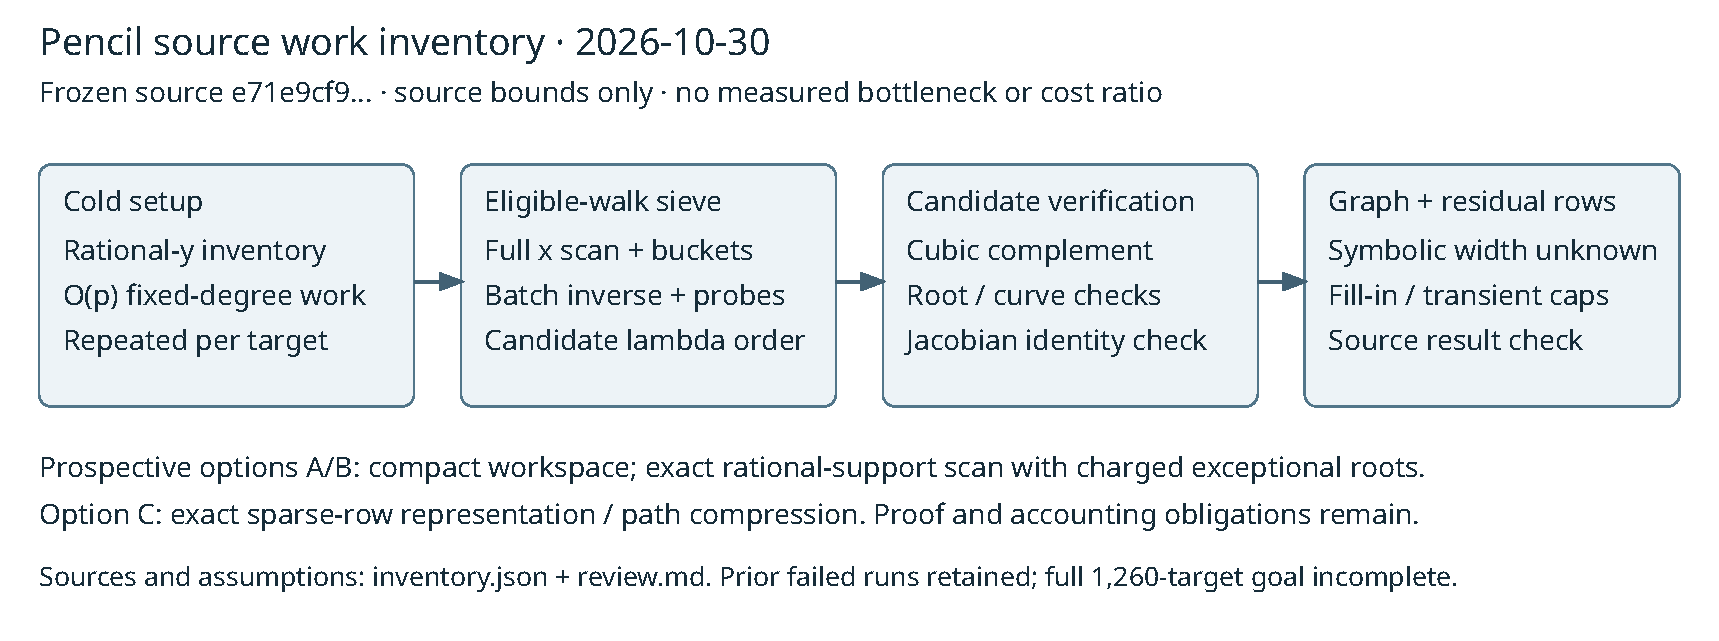
\includegraphics[width=\linewidth]{workflow-figure.pdf}

\textbf{Conditional source bounds at $p=186379$.} If all sixteen walks reach the degree-two sieve, full-x loops visit $16p=2,982,064$ positions. Two subsequent bucket passes visit $32p=5,964,128$ buckets. Earlier termination reduces these counts. They exclude setup, ordinate probes, polynomial coefficient work, assertions, sparse maps and allocation. They cannot identify which phase caused a timeout.

On the intended 64-bit ABI, a 24-byte vector header gives $24p=4,473,096$ bytes for bucket headers per sieve. This excludes element buffers and allocator overhead; it is not measured RSS. Ordinary probes are at most $2p$; the smooth genus-2 affine-point bound is $p+\lfloor4\sqrt p\rfloor=188,105$ under the stated curve hypotheses. Exceptional roots of degree-two $u$ number at most two.

\textbf{Complement and graph costs.} Complement verification uses fixed-degree polynomial arithmetic, not a field-wide root scan. It still charges exact division, root/curve checks and Jacobian verification. Size-balanced graph trees bound parent depth, but symbolic offset width remains unknown. For $S$ protected small columns, dense fill-in permits $O(S^2\log S)$ tree-map work per residual row and $O(S^2)$ retained basis size before caps. These are worst-case source bounds, not observed widths. A coefficient cap is not a whole-memory or wall-time bound; pending constraints and graph storage remain relevant.
\newpage
{\Large Prospective changes and proof obligations}\par
\textbf{A. Compact reusable sieve workspace.} Replace per-bucket vector allocations with bounded root slots or a flat buffer, plus a touched-index list. Preserve every exceptional append, candidate lambda order and verifier root order. Establish valid-input bucket cardinality, detect unsupported overflow, prove reset correctness and charge all copies/initializations. This changes instrument accounting and needs new source bindings.

\textbf{B. Rational-support iteration.} Ordinary x values without rational ordinates cannot produce a point-derived candidate. Iterate the existing rational-x inventory and separately find every root of quadratic $u$. Prove root completeness, handle repeated and exceptional roots exactly, preserve ordering where required, and charge root finding, inversions and deduplication. This remains generally $O(p)$ and has no claimed speedup.

\textbf{C. Exact sparse arithmetic.} Sorted sparse rows can replace repeated tree-map updates with merge-based updates; symbolic path compression may avoid repeated reconstruction. Preserve row space, signs/scales, smallest-pivot order, cancellation, transient working-cap behavior and retained pending rows. Checking only final row size is not equivalent to the existing intermediate cap checks. Charge compression and conversion work. Changes to partition, pivots or relation admission require a distinct protocol.

\textbf{PR 2935 boundary.} Its isolated early-rejection fork moves the root-count guard before complement computation. The retained static proof bounds skipped complements by two per eligible sieve, at most 32 over sixteen walks, assuming a valid smooth odd-characteristic quintic and degree-two Mumford input. It neither removes field-wide scans nor controls sparse fill-in. Its software fixtures supply no measured timeout remedy or performance ratio.

\textbf{Concrete next non-execution work.} Specify exact compact-bucket invariants and ordering, then build an isolated equivalence prototype with complete primitive ledgers. Separately inspect sparse fill-in/cap semantics. Any future progress observation must distinguish a censored partial prefix from completed costs; all setup, verification, root finding, graph work and unsuccessful work remain charged.

\textbf{Sources.} The unchanged full review is \texttt{review.md}; machine fields and source hashes are adjacent. Source root: \path{research/pencil_large_prime_20261029/}. Relevant files: \path{src/native_solver.rs} (824,850,1018,1311,1330), \path{src/lib.rs}, \path{src/collector.rs}, \path{src/residual.rs}; study README references prior Markowitz evidence. The early-rejection README and static bound were inspected without execution.

Gaudry--Theriault--Thome, February 2005, sections 2.3/3.1:
\url{https://cacr.uwaterloo.ca/techreports/2004/corr2004-29.pdf}.
Its coefficient-aware graph model informs the comparison, but its genus-at-least-three complexity theorem is not transferred to this genus-two pencil stream.

\textbf{Reporting limit.} No new result is substituted for prior failures, no timing qualification is granted, and no execution authorization follows from this source inventory. All candidate options remain unmeasured.
\end{document}
